\documentclass[12pt, letterpaper]{article}
\usepackage{graphicx}
\usepackage{booktabs}
\usepackage{float}


\title{A study on temporary impact and the Almgren-Chriss Model, an optimal order execution strategy}
\author{Chaitanya Agarwal}
\date{29 July 2025}


\begin{document}
\maketitle


\section{Modeling temporary impact $g_t(x)$}

We know, the temporary impact function $g_t(x)$ can be defined as the amount of slippage that occurs if $x$ orders are placed at the current time $t$. To effectively model $g_t(x)$, I analyzed the given MBP-10 snapshots of three companies, namely CoreWeave Inc(CRWV), JFrog Ltd(FROG), and SoundHound AI Inc(SOUN). Each snapshot provides the top ten bid and ask price-size pairs, from which I compute the mid-price $m_t$ and the spread. For each snapshot, I then "walk" the ask book, filling shares at successive price levels until \(x\) shares are filled. Slippage can then be calculated as:

\[g_t(x) \;=\;\frac{1}{x}\sum_{k=1}^{K}\bigl(p_k - m_t\bigr)\,\Delta x_k\]



For my initial simulations, I considered the following order sizes \newline $\{5, 50, 100, 500, 1000\}$ to get a rough sense of the shape of the slippage curves. After plotting the median slippage curves on log-log axes[Figure 1], we observe that for CRWV and FROG, slippage grows with order size. 
However, slippage remains flat for SOUN until larger order sizes($x  \geq 1000$). To capture a more representative curve for SOUN, I used a log-spaced grid of size 6 from 50 to 5000 shares(which increased the filesize from 3.38GB to 4.45GB).



\begin{figure}[h!] % 'h' means here
    \centering
    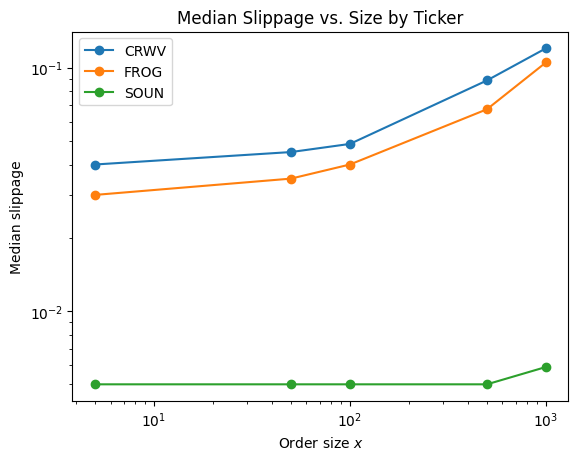
\includegraphics[width=0.78\textwidth]{res/images/median_slippage_small_grid.png} % Adjust width as needed
    \caption{Median Slippage for fixed grid}
    \label{fig:slippage_fixed_grid}
\end{figure}



\begin{figure}[h!] % 'h' means here
    \centering
    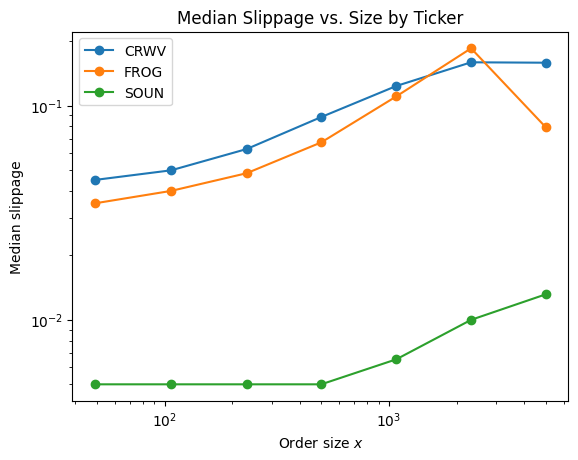
\includegraphics[width=0.78\textwidth]{res/images/median_slippage_med_grid.png} % Adjust width as needed
    \caption{Median Slippage for log-spaced grid}
    \label{fig:slippage_log_grid}
\end{figure}


The updated median slippage curves[Figure 2] now show SOUN rise sharply as the order size increases past 1000. The curves exhibit a concave trend where smaller order sizes incur a very small cost. If the order size was to be doubled, the increase in slippage would be far less than twofold. From my research, this behaviour points us towards two potential models:
\begin{itemize}
    \item \textbf{Linear}: $g(x) = \beta x$, which will serve as my baseline.
    \item \textbf{Power-law}: $g(x) = \alpha x^\gamma$, which exhibits concavity similar to the slippage curves.
\end{itemize}



I fit the aforementioned models to the median slippage data and report the estimated parameters, RMSE, and $R^2$ for the models, proving that power-law fits significantly better than any linear model.

\begin{table}[h!]
\centering
\begin{tabular}{lrrr} 
\toprule
Ticker & $\beta$ & RMSE & $R^2$ \\
\midrule 
CRWV  & $4.30\times10^{-5}$ & $3.407\times10^{-3}$ & $-0.6382$ \\
FROG  & $3.10\times10^{-5}$ & $4.483\times10^{-3}$ & $-0.8701$ \\
SOUN  & $3.00\times10^{-6}$ & $1.400\times10^{-5}$ & $-0.5688$ \\
\bottomrule
\end{tabular}
\caption{Linear fit results.}
\end{table}

\begin{table}[h!]
\centering
\begin{tabular}{lrrrr}
\toprule
Ticker & $\alpha$ & $\gamma$ & RMSE & $\mathrm{R}^2$ \\
\midrule
CRWV  & $1.2402\times10^{-2}$ & $0.3144$ & $1.42\times10^{-4}$ & $0.9649$ \\
FROG  & $1.1103\times10^{-2}$ & $0.2940$ & $1.393\times10^{-3}$ & $0.6835$ \\
SOUN  & $1.7750\times10^{-3}$ & $0.2112$ & $2.00\times10^{-6}$ & $0.7733$ \\
\bottomrule
\end{tabular}
\caption{Power-law fit results.}
\end{table}

\section{Order Execution Strategy}

2 pages at most.




\end{document}
